\documentclass{article}
\usepackage{graphicx} % Required for inserting images
\usepackage[margin=0.75in]{geometry}
\usepackage{xcolor}
\title{PH.140.644 Note -- In Class}
\author{Moran Guo}
\date{August 2024}

\begin{document}

\maketitle

\section{Aug 29th}
\subsection{Linear Model}
Consider a linear model: $$\hat{f}(X) = \hat{\beta}_0 + \hat{\beta}_1 X + \hat{\beta}_2 X + \hat{\beta}_3 X + \hat{\beta}_4 X + \hat{\beta}_5 X$$

How do we simplify it?\\

1. Sparsity of the parameters: Removing one (or more) variables.\\

2. Use non-linear models to re-model the outcome variable.\\

\noindent Flexibility vs. Interpret-ability\\

Increasing the flexibility \textbf{generalize the model}, but makes the model \textbf{harder to interpret}. -- How do we keep a balance between these two?\\

It seems that methods such as Trees and Generalized Additive Models keep a good balance between these two.\\

\noindent \textbf{Assessing Model Accuracy}\\

We could compute the Avg. MSE over training set ($\mathrm{Tr}$): $$\mathrm{MSE_{Tr}} = \mathrm{Ave_{i \in Tr}}[y_i - \hat{f}(x_i)]^2,$$

but this may be biased toward more over-fit models. Instead, we should use a new test data $\mathrm{Te} = \{x_i, y_i\}_1^M$ and calculate $$\mathrm{MSE_{Te}} = \mathrm{Ave_{i \in Te}}[y_i - \hat{f}(x_i)]^2.$$

In reality, the scenario is much more complex about how to decide the training and testing sets.

(If it's binary or classification problems, we could look at False Negative rate, False Positive rate, or misclassification \%).
\newpage
\begin{figure}[h!]
    \centering
    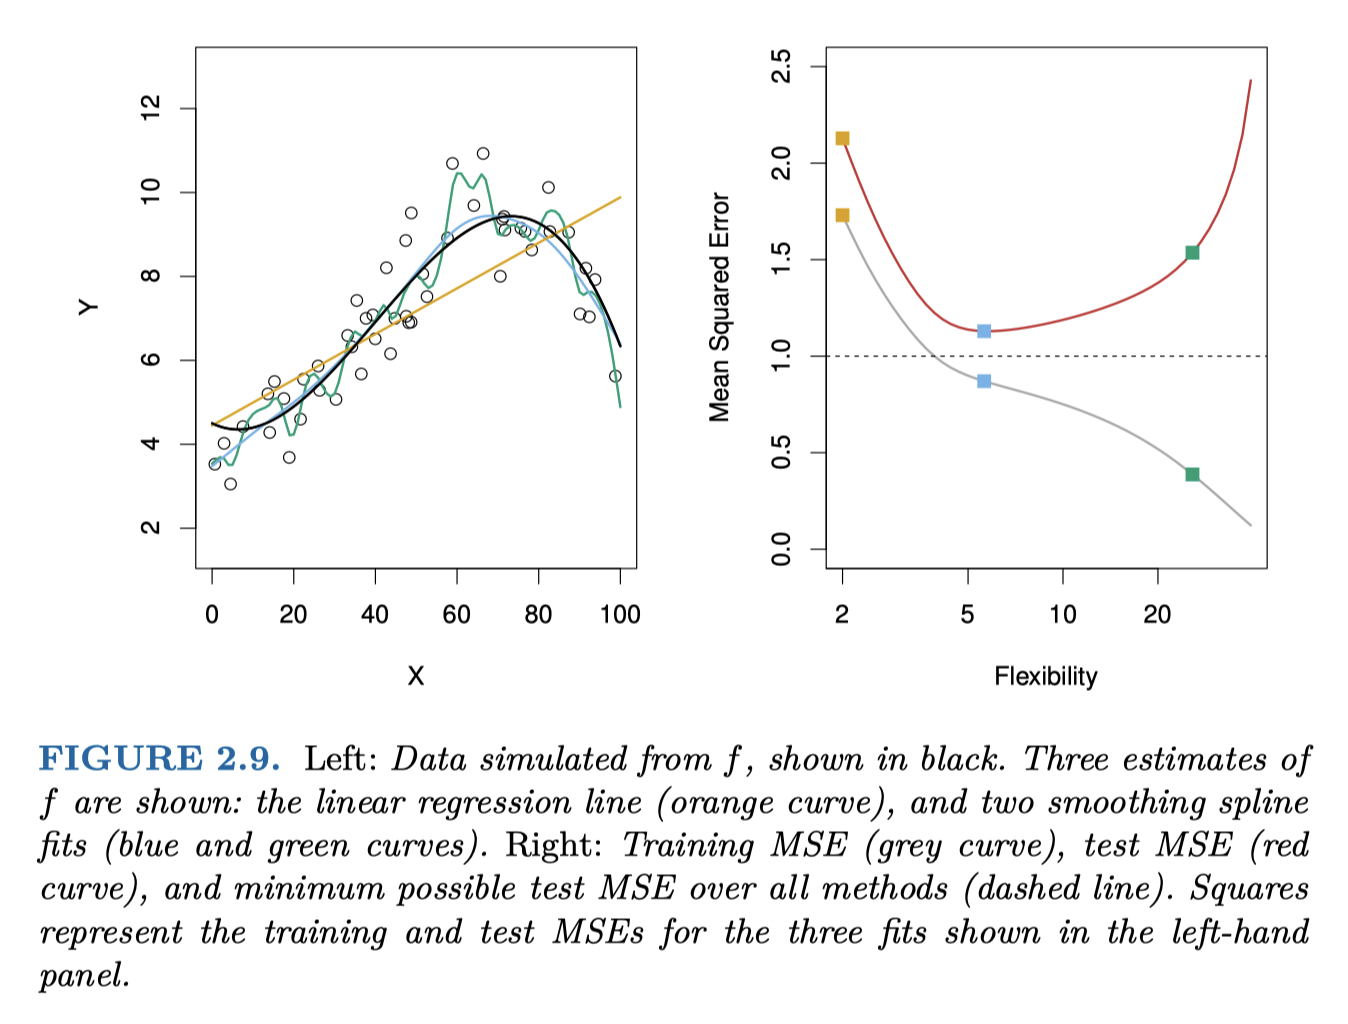
\includegraphics[width=0.75\linewidth]{Training_vs._Testing.png}
    \label{fig:train-vs-test}
\end{figure}

The \textcolor{blue}{blue} smoothing spline fit seems to perform the best across all three models. The \textcolor{green}{green} curve seems to have too much degrees of freedom by increasing the complexity of the model, which over-fits. In reality we are often time observing this U-shaped curve, where the overall MSE decreases when the complexity increase, but when the model is too complex, the $\mathrm{MSE_{Tr}}$ increases.\\

\noindent \textbf{Bias-Variance Trade-off}

Suppose we fit a model $\hat{f}(x)$ to training data $\mathrm{Tr}$, and let $(x_0, y_0)$ be an observation from the population. Then we have $$E\Big(y_0 - \hat{f}(x_0)\Big)^2 = \mathrm{Var}(\hat{f}(x_0)) + \Big[\mathrm{Bias}(\hat{f}(x_0))\Big]^2 + \mathrm{Var}(\epsilon).$$

\begin{figure}[h!]
    \centering
    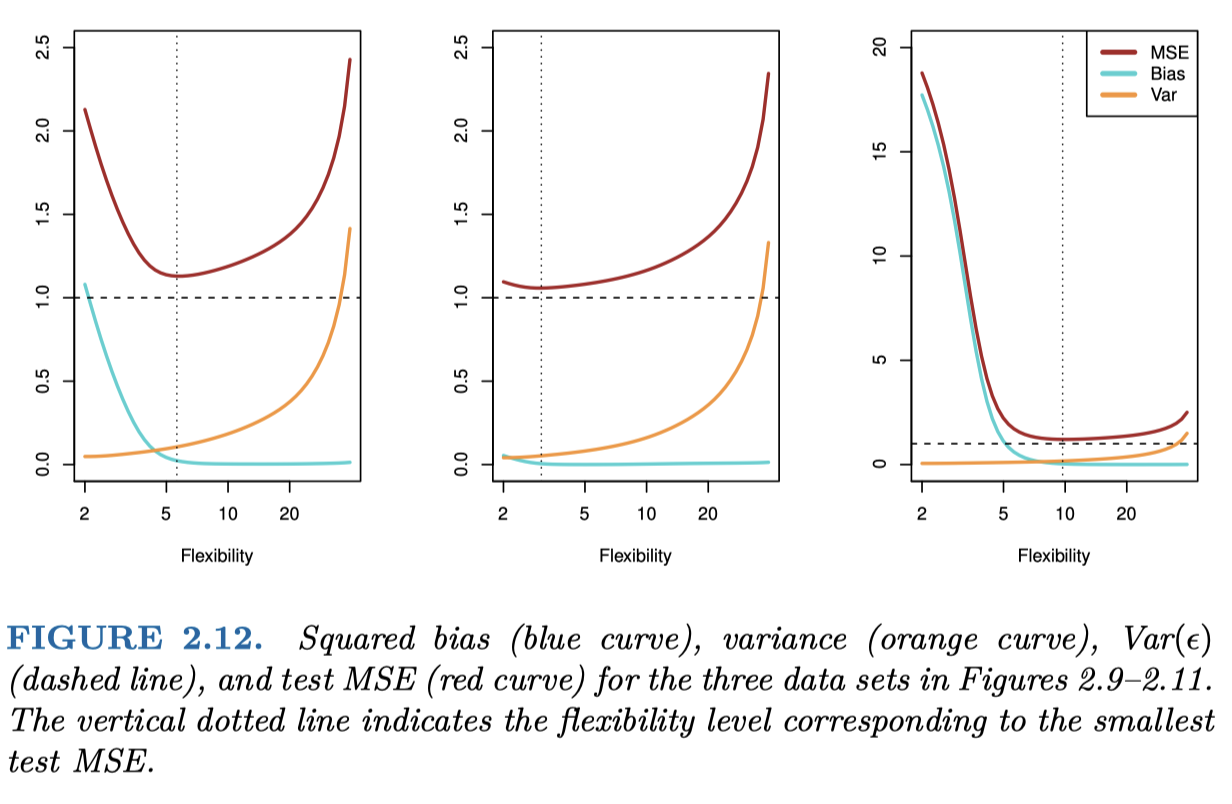
\includegraphics[width=0.75\linewidth]{bias_variance_tradeoff.png}
    \label{Bias-variance-tradeoff}
\end{figure}

As we are using more flexible model, the variance will increase and bias will decrease. But we generally have local minima to find the $\mathrm{MSE_{\min}}$.\\

\noindent \textbf{Classification Problem}

Response variable $Y$ is qualitative. Goal:
\begin{enumerate}
    \item Build a classifier $C(X)$ that assigns a class label from $\mathcal{C}$ to an unlabeled observation $X$.
    \item Assessing the uncertainty in each classification.
    \item Understand the roles of different predictors among $X$.
\end{enumerate}

To find the ideal $C(X)$, for $K$ elements in $\mathcal{C}$ numbered $1, 2, \cdots, K$. Let $$p_k(X) = \mathrm{Pr}(Y=k \vert X = x), k \in [1,K].$$

These are the conditional class probabilities at $x$; Then the \textbf{Bayes optimal classifier} at $x$ is $$C(x) = j$$  if $$p_j(x) = \max\{p_k(x)\}, k \in [1,K].$$\\

Nearest-neighbor averaging can also be used, especially when data is sparse.\\

\noindent \textbf{How good the model is} (classification model)?

Misclassification error rate: $$\mathrm{Err_{Te}} = \mathrm{Ave_{i \in Te}}I[y_i \neq \hat{C}(x_i)]$$

Pay attention to \textbf{selection bias} when having an \textbf{extremely low} misclassification rate.\\

\noindent \textbf{K-nearest Neighbors}
\begin{figure}[h!]
    \centering
    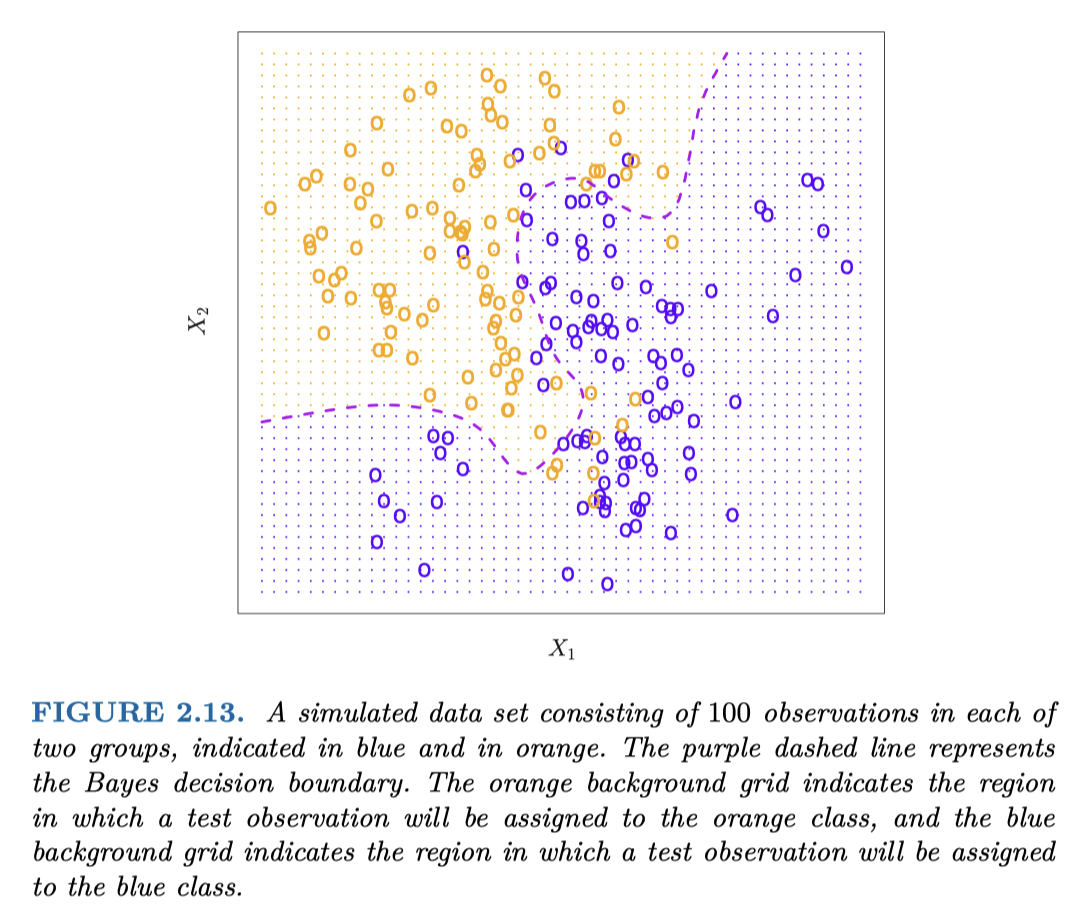
\includegraphics[width=0.60\linewidth]{KNN.png}
    \label{fig:KNN}
\end{figure}

There are some misclassified data which could be observed from the graph.

\newpage

\begin{figure}[h!]
    \centering
    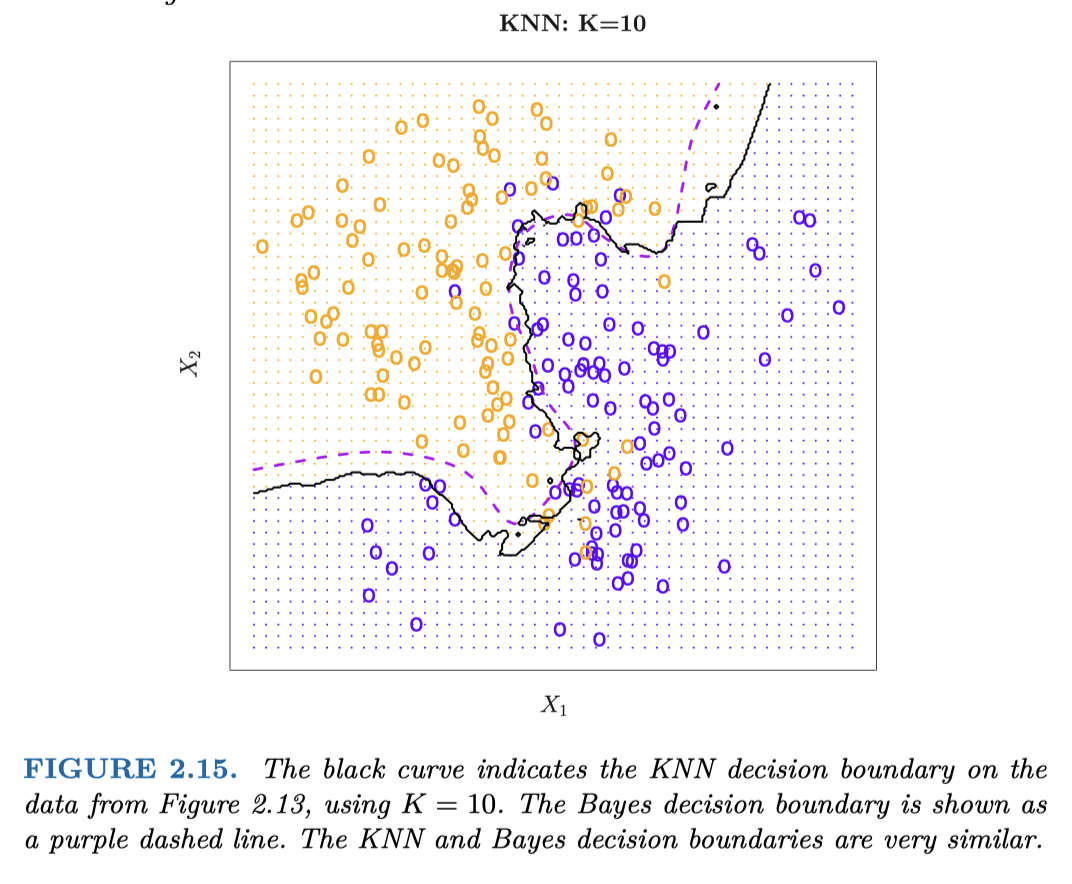
\includegraphics[width=0.5\linewidth]{KNN_10.png}
    \label{fig:KNN-10}
\end{figure}

The black curve is the estimate of the K-Nearest Neighbor with $K = 10$. The boundary is established by sampling the $10$ nearest data points of a particular data point and observe the majority color of those points.

\begin{figure}[h!]
    \centering
    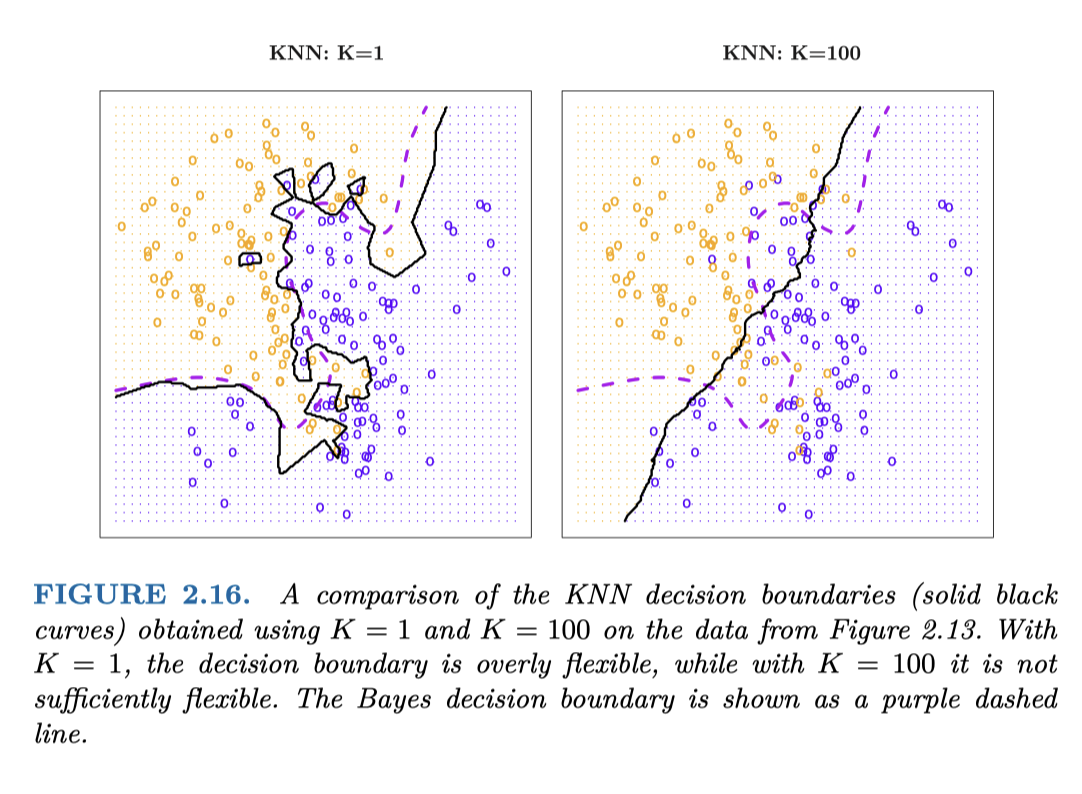
\includegraphics[width=0.75\linewidth]{KNN_compare.png}
    \label{fig:KNN-compare-1-100}
\end{figure}

The $K=1$ KNN estimate gives too much complexity which can be observed from the under-smoothed curve and islands emerged. Instead, if we use $K=100$ KNN, this model gives too little complexity which we cannot learn much from the model.
\newpage
\begin{figure}[h!]
    \centering
    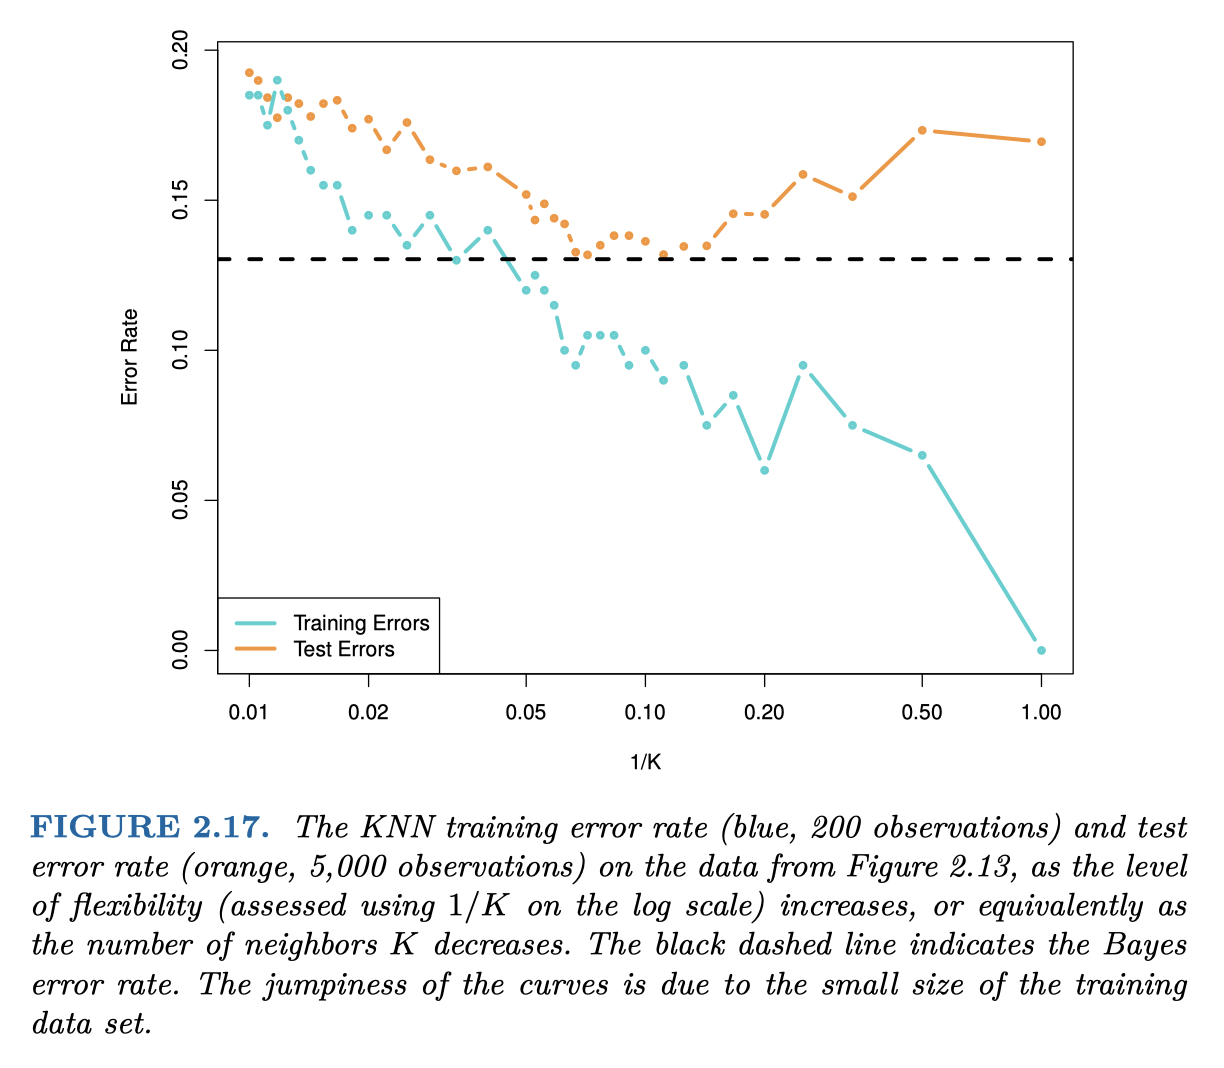
\includegraphics[width=0.75\linewidth]{Training_testing_error.png}
    \label{fig:training-testing-error}
\end{figure}

The training errors goes down as $K$ increases. However, the testing errors generally obey an U-shaped curve. We can see that $K=10$ is optimal here.

\section{Sep 3rd}

\subsection{Linear Regression}

Linear regression is a simple approach to supervised learning. It assumes that the dependence of $Y$ on $X_1, X_2, \dots, X_p$.\\

\noindent \textbf{Variable Selection}\\

Strategy 1:
Try one variable at a time, and calculate the training error.\\

For multiple variables, we consider \textit{all subsets} of the variables to select the \textbf{best} \textit{subset} of the combination of variables. However, there are too much $(2^p)$ of combinations, so it is not realistic.\\

So we need an automated approach that searches through a subset of them. (Refer to book pp. 79)

\subsection{Classification}

Qualitative variables in an unordered set $\mathcal{C}$, e.g., eye color, email, etc.\\

Given: feature vector $X$ and qualitative response $Y$ taking values from $\mathcal{C}$, classification is to:\\

Build a function $C(X)$ s.t. takes feature vector $X$ as input and output predicted $Y$.

\newpage

\begin{figure}[h!]
    \centering
    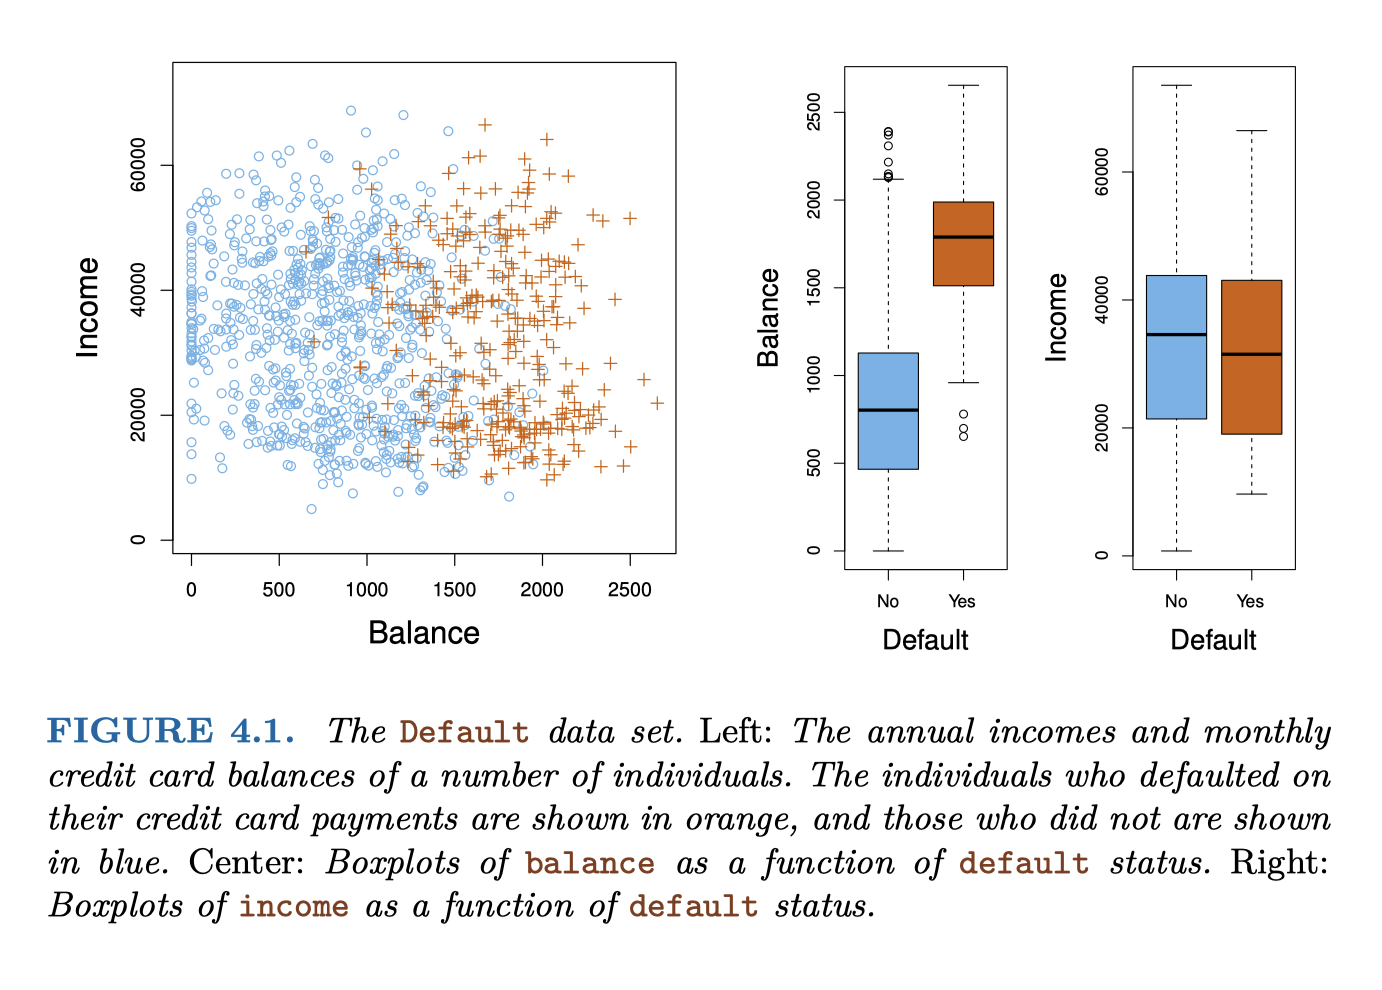
\includegraphics[width=0.75\linewidth]{Classification_income_vs_balance.png}
    \label{fig:income-vs-balance}
\end{figure}

Clients that have a high balance are associated with higher chance (observed) of default, compared to those with a low balance.\\

Can we perform a simple linear regression to predict a binary outcome?
E.g., perform a regression of $Y$ on $X$ and classify as ``Yes'' (or ``No'') if $\hat{Y} > 0.5$? -- Yes we can.\\

However, linear regression does not provide meaningful estimates of $\mathrm{Pr}(Y \vert X)$, compared to logistic regression.

\subsection{Logistic Regression}

$p(X) = \mathrm{Pr}(Y = 1 \vert X)$, consider using $\color{red}{balance}$ to predict $\color{red}{default}$. Logistic regression uses $$p(X) = \frac{e^{\beta_0 + \beta_1 x}}{1 + e^{\beta_0 + \beta_1 x}} \Longrightarrow \frac{p(X)}{1-p(X)} = e^{\beta_0 + \beta_1 x}.$$

$\displaystyle \frac{p(X)}{1 - p(X)}$ is called \textbf{odds}.\\

We uses Maximum Likelihoods to estimate the parameters:

$$\displaystyle\ell(\beta_0, \beta_1) = \prod_{i:y_i = 1}p(x_i)\prod_{i:y_i = 0}\Big(1 - p(x_i)\Big)$$

\begin{figure}[h!]
    \centering
    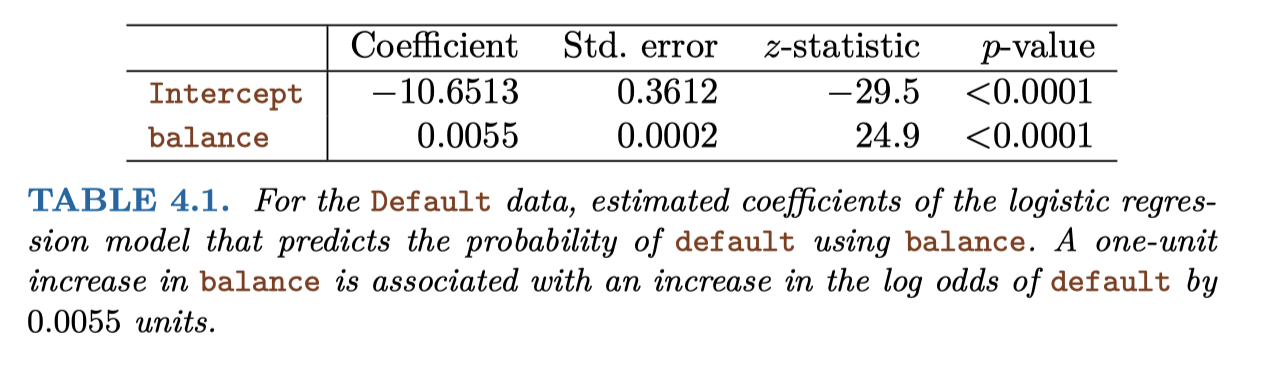
\includegraphics[width=0.75\linewidth]{GLM_result.png}
    \label{GLM-logistic}
\end{figure}

We can start to make a prediction now. From the table above we get $\hat{\beta}_0 = -10.6513$ and $\hat{\beta}_1 = 0.0055$. So 

\newpage

\begin{figure}
    \centering
    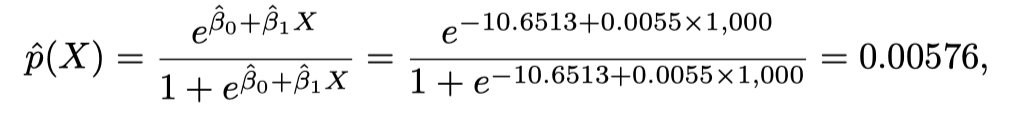
\includegraphics[width=0.75\linewidth]{calculation_logistic.png}
    \label{calculation-logistic}
\end{figure}

with a balance of $\$1000$.

\subsection{Confounding}

\subsection{Multiple Logistic Regression}

$$\mathrm{Pr}(Y = k \vert X = x) = \frac{e^{\beta_{k0} + \beta_{k1} + \dots + \beta_{kp}x_p}}{1 + \sum_{l=1}^{K=1}e^{\beta_{l0} + \beta_{l1x_1} + \dots + \beta_{lp x_p}}}$$

To predict the most likely class for multiple classes.

\subsection{Discriminant Analysis}

The approach is to model the distribution of $X$ in each of the class separately, then uses $\color{green}{\mathrm{Bayes \ Theorem}}$ to obtain $\mathrm{Pr}(Y \vert X)$.

$$\mathrm{Pr}(Y = k \vert X = x) = \frac{\mathrm{Pr}(X = x \ \vert\ Y = k) \cdot \mathrm{Pr}(Y = k)}{\mathrm{Pr}(X = x)}$$

Note that the denominator is \textbf{not dependent on} $k$.\\

For discriminant analysis we write 
$$\mathrm{Pr}(Y = k \vert X = x) = \frac{\pi_k f_k(x)}{\sum_{l=1}^K \pi_l f_l(x)}$$

Why discriminant analysis?\\

The logistic regression model are \textbf{unstable when the classes are well-separated}. Linear discriminant analysis does not suffer from this problem.\\

If $n$ is small and the distribution of the predictors $X$ is approx. normal in every classes, then the linear discriminant model is more stable than the logistic regression model.\\

Also, it is popular when we have more than two response classes.\\

\textbf{Linear Discriminant Analysis when $p = 1$}

From Gaussian density, $$f_k(x) = \frac{1}{\sqrt{2\pi}\sigma_k}e^{-\frac{1}{2}\Big(\frac{x - \mu_k}{\sigma_k}\Big)^2}$$

We assume that all the $\sigma_1 = \sigma_2 = \dots = \sigma_k$.

Then we find that $$p_k(x) = \frac{\pi_k \frac{1}{\sqrt{2\pi}\sigma}e^{\Big(- \frac{1}{2\sigma^2}(x - \mu_k)^2\Big)}}{\sum_{l=1}^K \pi_l \frac{1}{\sqrt{2\pi}\sigma}e^{\Big(- \frac{1}{2\sigma^2}(x - \mu_l)^2\Big)}}.$$

\section{Sep 5th}

\textit{Control the size of the submitted PDF file.}

\subsection{Estimate the parameters}
Start from 
$$\mathrm{Pr}(Y = k \vert X = x) = \frac{\pi_k f_k(x)}{\sum_{l=1}^K \pi_l f_l(x)}$$

We estimate $\displaystyle\hat{\pi}_k = \frac{n_k}{n}$, $\displaystyle\hat{\mu}_k = \frac{1}{n_k}\sum_{i: y_i = k}x_i$, $\displaystyle\hat{\sigma}^2 = \frac{1}{n - K}\sum_{k=1}^K \sum_{i: y_i = k}(x_i - \hat{\mu}_k)^2 = \sum_{k=1}^K \frac{n_k -1}{n - K}\cdot \hat{\sigma}_k^2.$\\

We are trying to ask the question ``is this subject looks more alike a subject who didn't defaulted or did defaulted?''

\subsection{LDA with $p$-dimensional $(p > 1)$}

From the multivariate Gaussian density:

\begin{figure}[h!]
    \centering
    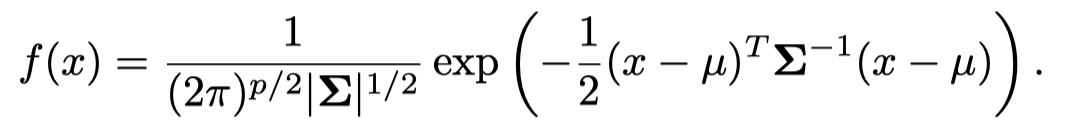
\includegraphics[width=0.75\linewidth]{Multi_Gaussian.png}
    \label{multi_gaussian}
\end{figure}

We construct the Bayes classifier as $$\delta_k(x) = x^T \Sigma^{-1}\mu_k - \frac{1}{2}\mu_k^T \Sigma^{-1}\mu_k + \log \pi_k$$

$\delta_k(x)$ is a linear function despite its complex form.

\begin{figure}[h!]
    \centering
    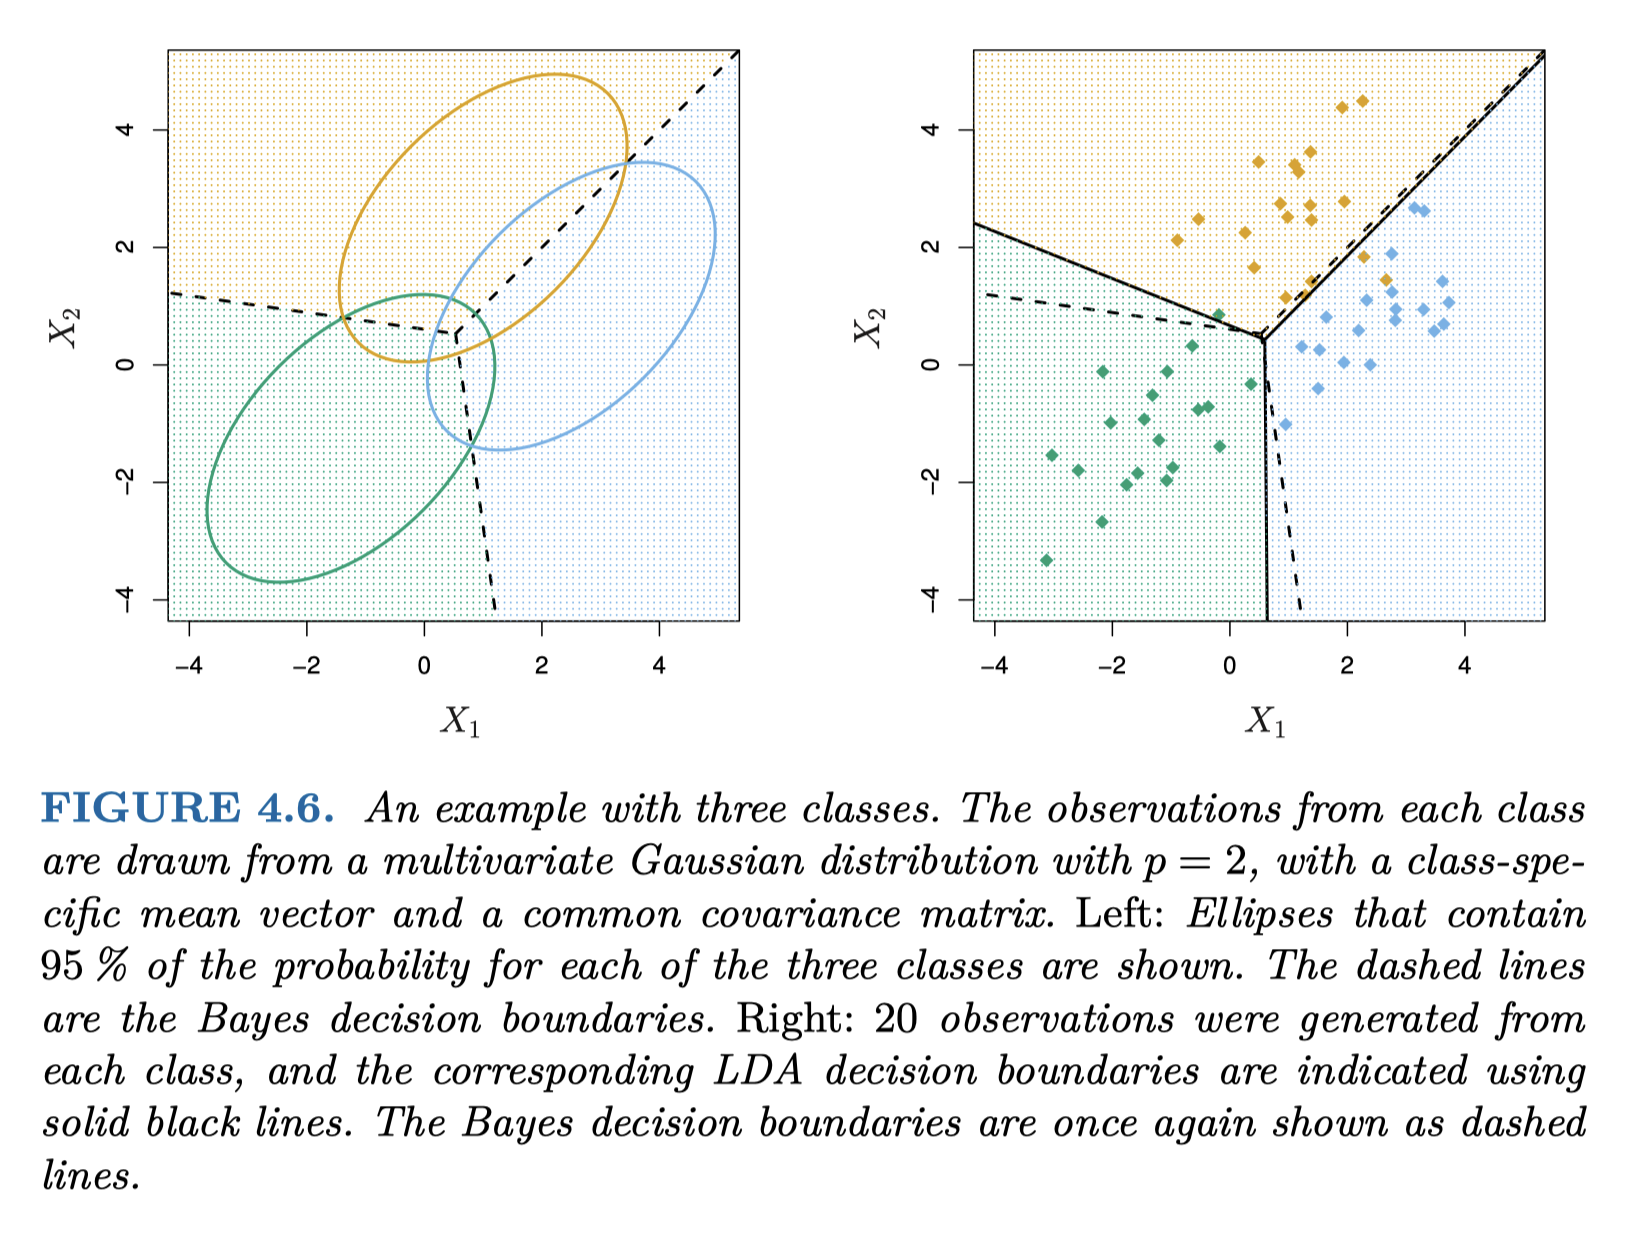
\includegraphics[width=0.75\linewidth]{Bayes_boundaries.png}
    \label{Bayes_boundaries}
\end{figure}

Deviations between the true and estimated Bayes classifier boundaries exist. Dashed lines indicate the Bayes decision boundaries.

\newpage

\begin{figure}
    \centering
    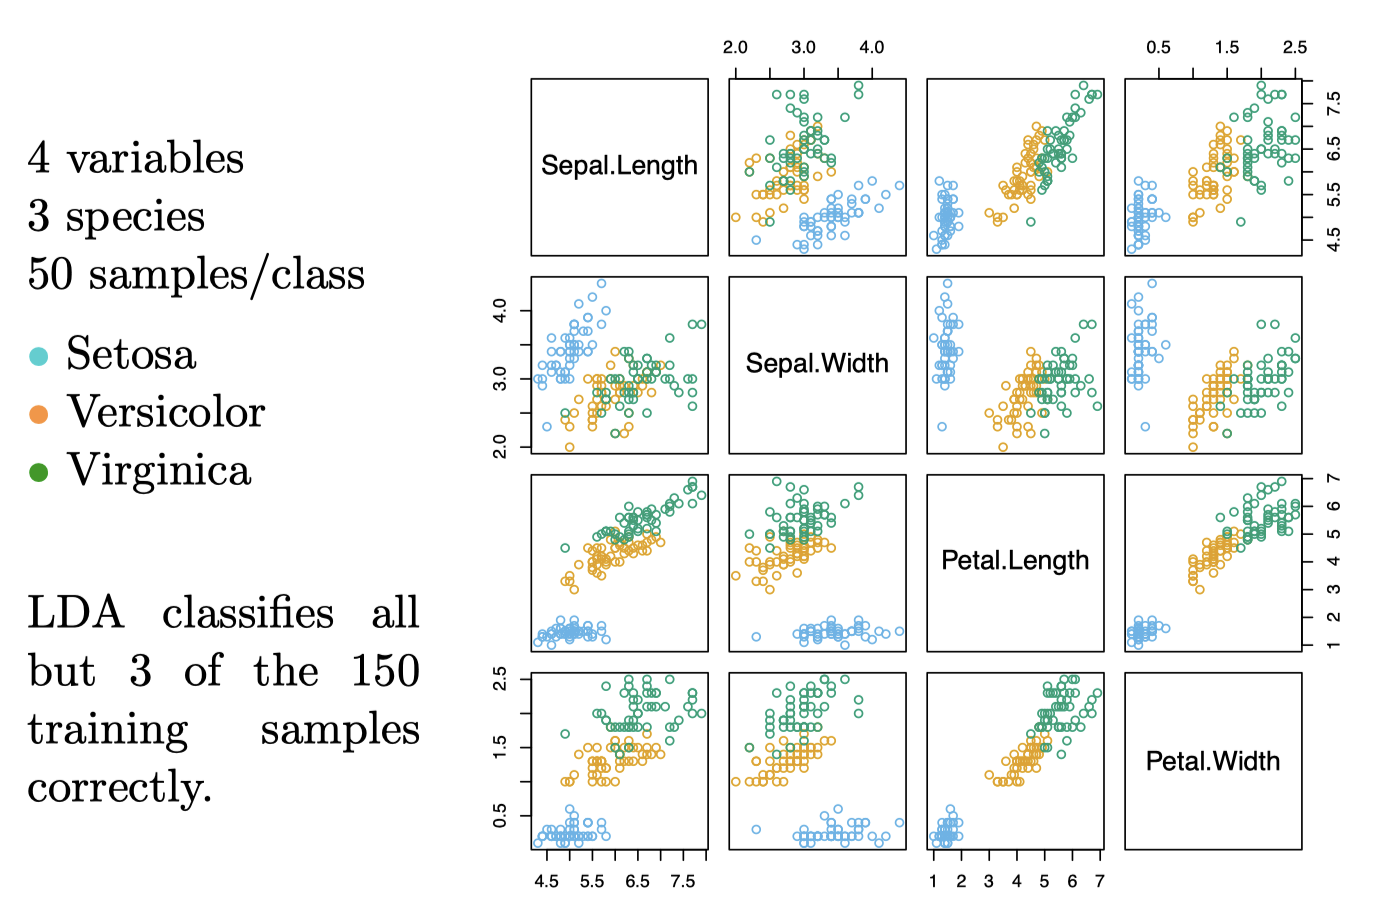
\includegraphics[width=0.75\linewidth]{Iris_data.png}
    \label{Iris_data}
\end{figure}

From the figure, we can observe that $\color{blue}{Setosa}$ species separate well compared to the rest two species.

\begin{figure}[h!]
    \centering
    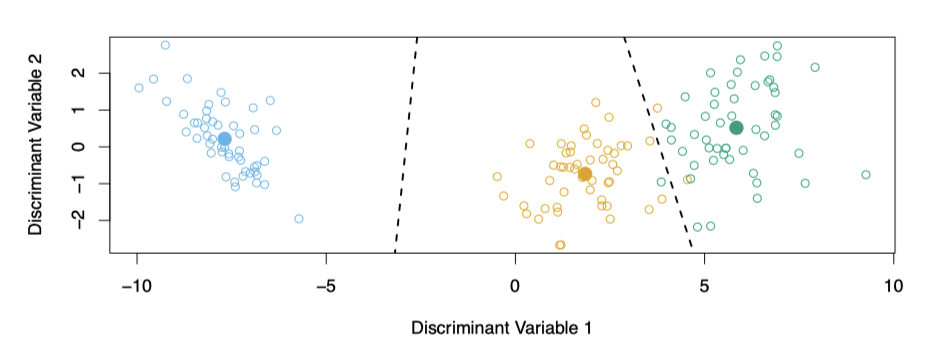
\includegraphics[width=0.75\linewidth]{Discriminant_plot.png}
    \label{Discriminant_plot}
\end{figure}

From the data, we first calculate \textbf{Discriminant Variable} $1$ and $2$ from the variables of the data provided. Then we plot them on the Fisher's discriminant plot and assign to specific classes.

From $\hat{\delta}_k(x)$ we can turn these into estimates of probabilities: $$\widehat{\mathrm{Pr}}(Y = k \vert X = x) = \frac{e^{\hat{\delta}_k(x)}}{\sum_{l=1}^K e^{\hat{\delta}_l(x)}}.$$
\newpage
\begin{figure}[h!]
    \centering
    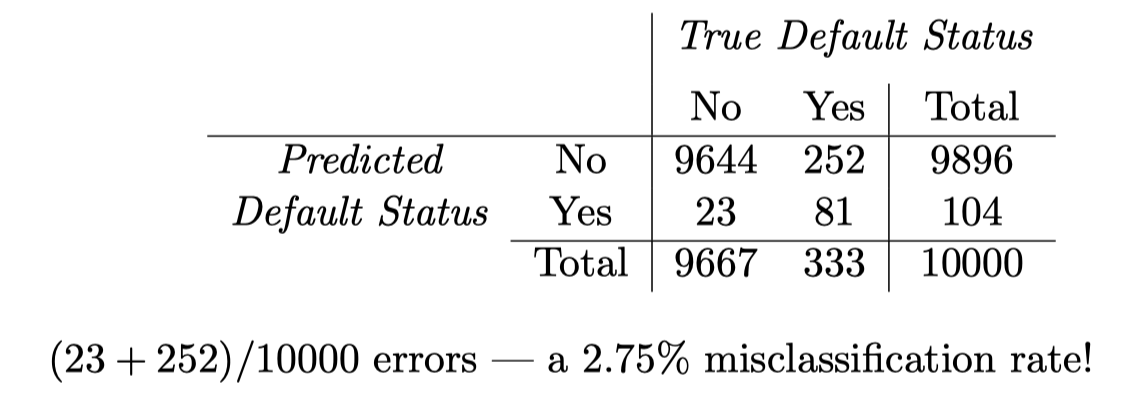
\includegraphics[width=0.75\linewidth]{Credit_data_LDA.png}
    \label{Credit_data_LDA}
\end{figure}

From the example, we have a $2.75\%$ misclassification rate.\\

Caveats:
\begin{enumerate}
    \item This is training error, may be overfitting.
    \item Notice the inbalance of the data. If we always classifies the data into ``non-default'' category, we only have a $3.33\%$ error rate.
    \item Among the 333 cases that are truly default, the model wrongly predicted a large majority of the cases $(252/333 = 75.7\%)$ as being not default. This is a high false negative rate.
\end{enumerate}

\begin{figure}[h!]
    \centering
    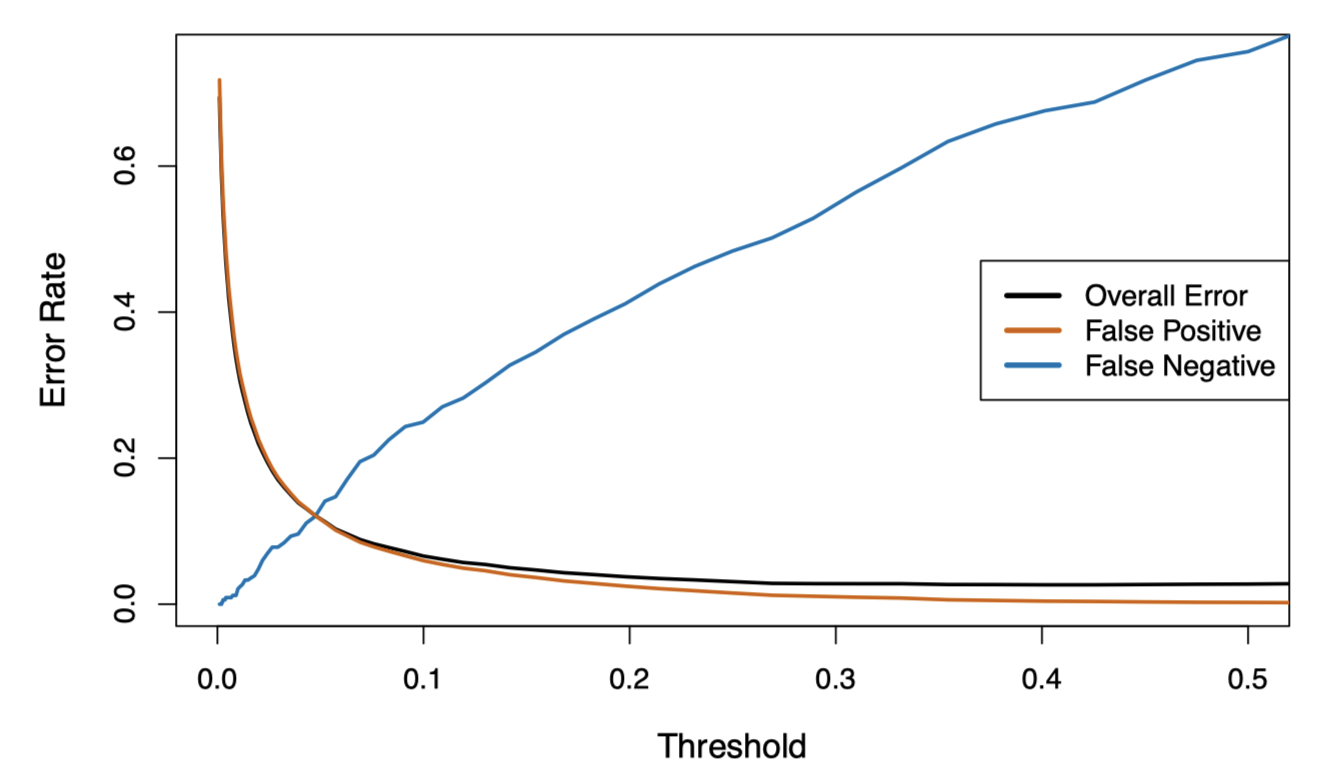
\includegraphics[width=0.75\linewidth]{FN_FP_tradeoff.png}
    \label{FN_FP_tradeoff}
\end{figure}

There is always a trade-off between reducing false negative and false positive rate. If we want to reduce one, the other will increase.

\newpage

\subsection{ROC Curve}

\begin{figure}[h!]
    \centering
    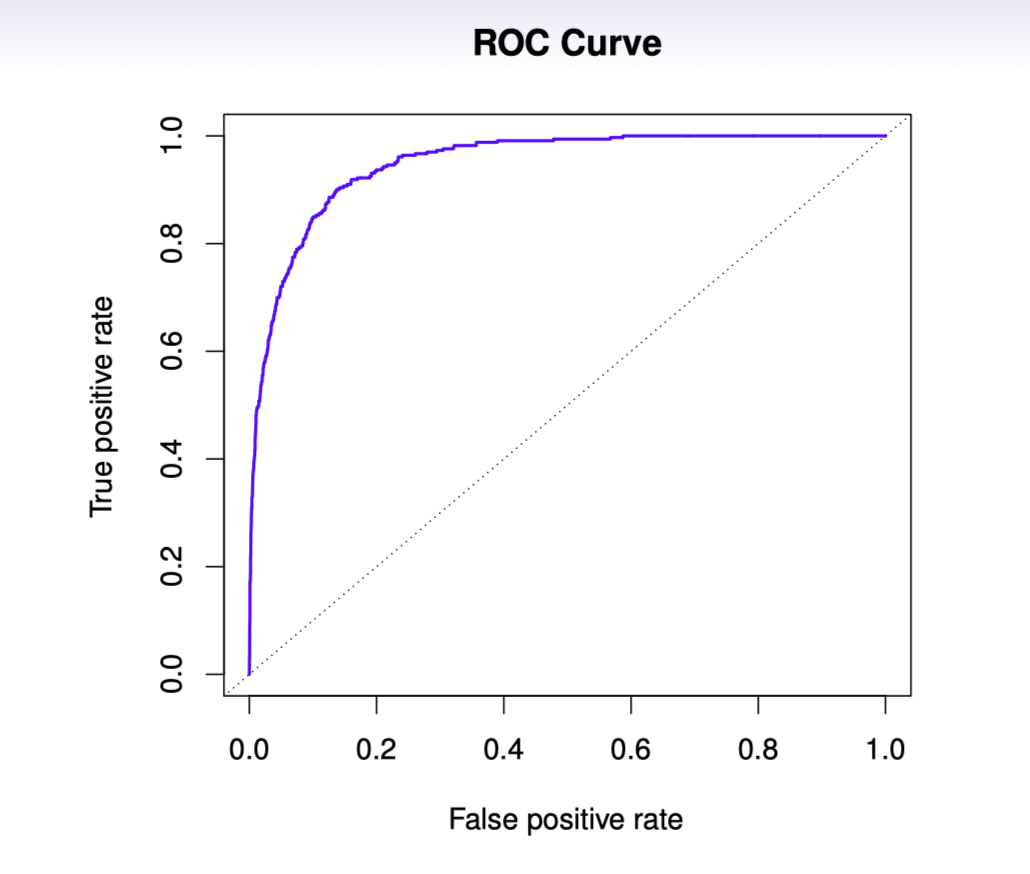
\includegraphics[width=0.5\linewidth]{ROC.png}
    \label{ROC}
\end{figure}

ROC curve allows for plotting false positive and true positive rates on the same plot and thus allows us to determine a \textit{threshold}. Sometimes we use \textit{AUC} (area under the curve) to evaluate the performance of the model, with the higher \textit{AUC} the better the performance.

\end{document}
